\section{Volumetric Rendering}
\label{section:volumetric-rendering}

\subsection{Definition}
\Gls{volumetricrendering} describes a technique for generating a visual representation of data that is stored in a 3D volume. 
This especically comes to use for visual effects that are volumetric in nature, like fluids, clouds, fire, smoke, fog and dust, which all are extremely difficult or even impossible to model with geometric primitives.
\\
In addition to rendering such effects, volumetric rendering has become essential to scientific applications like medical imaging, for which a typical 3D data volume is a set of 2D slice images acquired by a CT (computed tomography) or MRI (magnetic resonance imaging) scanner.
\emptyline
The data volume is also called a \textit{\gls{scalarfield}} or \textit{\gls{vectorfield}}, which associates a scalar or vector value, called \textit{\gls{voxel}} (short for \textit{volume element}), to every point in the defined space.
For a scalar field, it can be imagined like a 3D grid, where each point holds a single number. This number could, for example, represent the density of a cloud at that very point.

\subsection{Constant Step Ray Marching}
To actually render the volume data, a method called \textit{\gls{raymarching}} is used. With it, the surface distance of the volumetric data is approximated by creating a ray from the camera to the object for each fragment processed in the fragment shader. The ray is then extended into the volume of the object and stepped forward until the surface is reached.

\begin{figure}[H]
    \centering
    \begin{tikzpicture}[scale=0.7]
        \node[red] (p1) at (2.5,3) {};

        \draw[-{Latex[length=2mm]},cyan,shorten <=-4pt] (p1) node[below right]{stepped forward} -- (4.75,4.125);
        \node[cyan] at (3.0,3.25) {\textbullet};
        \node[cyan] at (3.5,3.50) {\textbullet};
        \node[cyan] at (4.0,3.73) {\textbullet};
        
        \node[red] at (p1) {\ding{53}};

        \draw (0,0) -- (5,0) -- (5,5) -- (0, 5) -- (0, 0);
        \draw (2,1) -- (7,1) -- (7,6) -- (2, 6) -- (2, 1);
        \draw (0,0) -- (2,1); \draw (5,0) -- (7,1); \draw (5,5) -- (7,6); \draw (0,5) -- (2,6); 

        \draw[red,shorten >=-4pt] (-1.5,1) node[below right]{camera ray} -- (p1);

    \end{tikzpicture}
    \captionof{figure}{Ray marching concept visualized.}
\end{figure}

\pagebreak
\noindent
In \gls{raymarching}, the algorithm only knows when it has reached the surface, or to be precise when it is inside the actual object volume.
\\
With this information, it is only possible to extend the ray in steps of a predefined length until the inside of the object is reached.
With a constant step, the approximation of the surface distance is exactly as precise as the size of the constant step.
\\
Once the ray is inside the actual volume, the functions returns the distance for this ray.

\begin{figure}[H]
    \centering
    \begin{tikzpicture}[scale=1.2]
        \tikzset{edge/.style = {-{Latex[length=3mm]}}}
        \tikzset{smalledge/.style = {-{Latex[length=1mm]}}}

        % ray
        \draw[edge] (0,2) node[above,sloped,xshift=1cm]{ray} -- (10,3);
        \node (1) at (2,2.2) {\textbullet};
        \node (2) at (3,2.3) {\textbullet};
        \node (3) at (4,2.4) {\textbullet};
        \node (4) at (5,2.5) {\textbullet};
        \node (5) at (6,2.6) {\textbullet};
        \node (6) at (7,2.7) {\textbullet};
        \node[cyan] (7) at (8,2.8) {\textbullet};

        % surf dist
        \draw[red] (2,1.5) -- (2.5,2) -- (4,1.8) -- (5,1.5) -- (7.4,2) -- (7.7,4) -- (9,4.3);

        % ray steps
        \draw[smalledge] (1) edge[bend left=60] node [left]{} (2);
        \draw[smalledge] (2) edge[bend left=60] node [left]{} (3);
        \draw[smalledge] (3) edge[bend left=60] node [left]{} (4);
        \draw[smalledge] (4) edge[bend left=60] node [left]{} (5);
        \draw[smalledge] (5) edge[bend left=60] node [left]{} (6);
        \draw[smalledge] (6) edge[bend left=60] node [left]{} (7);

        % returns text
        \draw[cyan, shorten <=-0.2cm] (7) -- (9,3.7) -- (11,3.7) node[xshift=-1cm,above]{function returns};
        
        \end{tikzpicture}
    \captionof{figure}{Traditional ray marching.}
\end{figure}

\noindent
An implementation of this algorithm can be seen in \autoref{lst:shader:raymarch:constantstep}. Note that the volume to be rendered in this example is just a simple sphere.
So in order to check if the ray is inside the volume, the function \lstinline[language=HLSL]{sphereHit()} is used.
\begin{lstlisting}[language=HLSL, numbers=left, caption=Implementation of a volume distance function for a sphere.,captionpos=b, label=lst:shader:raymarch:spherehit]
bool sphereHit(float3 position) {
    float4 sphere = float4(0, 1, 0, 1);
    return distance(sphere.xyz, position) < sphere.w;
}
\end{lstlisting}

\noindent
With that given, the raymarch function is implemented like so:

\begin{lstlisting}[language=HLSL, numbers=left, caption=Implementation of a ray march function with constant step.,captionpos=b, label=lst:shader:raymarch:constantstep]
fixed4 raymarch(float3 position, float3 direction)
{
    for (int i = 0; i < MAX_STEPS; i++)
    {
        if (sphereHit(position))
            return fixed4(1,0,0,1);
        
        position += normalize(direction) * STEP_SIZE;
    }
    
    return fixed4(0,0,0,1);
}
\end{lstlisting}


\pagebreak
\subsection{Traditional Ray Marching}
It is obvious to see that, for a constant step ray march to result in an accurate approximation of the surface distance, the step size is required to be relatively small.
This has a direct impact on performance and thus, is not a viable solution for the problem.
\\
In traditional \gls{raymarching}, an optimization for that has been developed. The algorithm does not blindly step forward, but instead tries to get as close to the real distance as possible.
After the volume is reached, the step size is decreased and the ray steps out of the volume again. It then tries to approximate the surface distance by stepping back and forth repeatedly in continuously smaller steps, thus converging towards the exact intersection.
Once the step size falls below a certain threshold, the distance approximation is assumed to be precise enough and the value is returned for that ray march.

\begin{figure}[H]
    \centering
    \begin{tikzpicture}[scale=1.2]
        \tikzset{edge/.style = {-{Latex[length=3mm]}}}
        \tikzset{smalledge/.style = {-{Latex[length=2mm]}}}

        % ray
        \draw[edge] (0,2) node[above,sloped,xshift=1cm]{ray} -- (10,3);
        \node (1) at (2,2.2) {\textbullet};
        \node (2) at (4,2.4) {\textbullet};
        \node (3) at (6,2.6) {\textbullet};
        \node[cyan] (4) at (8,2.8) {\textbullet};

        % surf dist
        \draw[red] (2,1.5) -- (2.5,2) -- (4,1.8) -- (5,1.5) -- (7.4,2) -- (7.7,4) -- (9,4.3);

        % reverse nodes
        \node[cyan] (5) at (7,2.7) {\textbullet};
        \node[cyan] (6) at (7.5,2.75) {\textbullet};

        % ray steps
        \draw[smalledge] (1) edge[bend left=60] node [left]{} (2);
        \draw[smalledge] (2) edge[bend left=60] node [left]{} (3);
        \draw[smalledge] (3) edge[bend left=60] node [left]{} (4);

        % rey reverse steps
        \draw[smalledge,cyan,shorten >=-0.1cm,shorten <=-0.1cm] (4) edge[bend left=60] node [left]{} (5);
        \draw[smalledge,cyan,shorten >=-0.1cm,shorten <=-0.1cm] (5) edge[bend left=60] node [left]{} (6);

        % close enough
        \draw[cyan, shorten <=-0.2cm] (6) -- (9,3.7) -- (11,3.7) node[xshift=-1cm,above]{step size small enough};
        
        \end{tikzpicture}
    \captionof{figure}{Traditional ray marching.}
\end{figure}

\noindent
As clearly visible, the traditional \gls{raymarching} ends up with a more precise result and the amount of steps per ray could be relatively lower, ultimately saving performance. 
\\
However, there is still an issue. The algorithm may jump in and out of the volume, even if it would already be precise enough, essentially taking unnecessary steps.

\begin{lstlisting}[language=HLSL, numbers=left, caption=Implementation of a traditional ray march function with converging surface distance approximation.,captionpos=b, label=lst:shader:raymarch:traditional]
fixed4 raymarch(float3 position, float3 direction)
{
    float stepSize = STEP_SIZE;
    float dirMultiplier = 1;
    for (int i = 0; i < MAX_STEPS; i++)
    {
        if (stepSize < MINIMUM_STEP_SIZE)
            return fixed4(1,0,0,1);

        if (sphereHit(position)) {
            // reduce step size by half and invert marching direction.
            stepSize /= 2;
            dirMultiplier = -1;
        } else {
            dirMultiplier = 1;
        }
        
        position += normalize(direction) * stepSize * dirMultiplier;
    }
    
    return fixed4(0,0,0,1);
}
\end{lstlisting}

\pagebreak
\subsection{Sphere Tracing}
An even better approach to approximate the intersection of the ray and the volume is called \textit{\gls{spheretracing}}. 
Instead of evaluating if the ray is inside the volume or not, an exact distance to the scene is measured. This distance is the minimum amount of space the algorithm can march along its ray without colliding with anything.
For that, a function group called \textit{\gls{sdf}s} is used.

\subsubsection{Signed Distance Functions}
A \gls{sdf} (SDF) returns the shortest distance from that a given point in space to some surface.
The sign of the returned value indicates wether that point is inside the surface or outside, hence the name.
\\
For example, the \gls{sdf} $f(p)$ for a point $p=(p_1, p_2, p_3)$ to the surface of a sphere $s=(s_1, s_2, s_3)$ with radius $R$ looks like this:
$$ f(p) = \sqrt{(s_1 - p_1)^2 + (s_2 - p_2)^2 + (s_3 - p_3)^2} - R $$

\noindent
This translates into a simple code snippet, mostly identical to the function \lstinline[language=HLSL]{sphereHit()} in \autoref{lst:shader:raymarch:spherehit}, except the distance is returned instead of a boolean.
\begin{lstlisting}[language=HLSL, caption=Implementation of a signed distance function for a sphere., label=lst:shader:raymarch:spheredistance]
float sceneSDF(float3 position) {
    float4 sphere = float4(0, 0, 0, 1);
    return distance(sphere.xyz, position) - sphere.w;
}
\end{lstlisting}

\noindent
With the sphere in the example being at the origin and having $R = 1$, a positive distance is returned for points outside the sphere and a negative distance if the point is inside the sphere.
\begin{lstlisting}[language=HLSL]
float d1 = sceneSDF(float3(2, 0, 0));   // d1 = 1.0
float d2 = sceneSDF(float3(0, 0.5, 0)); // d2 = -0.5
float d3 = sceneSDF(float3(5, -5, 5));  // d3 = 7.66
\end{lstlisting}

\subsubsection{Sphere Tracing with SDFs}
If the distance to the scene can be calculated with a \gls{sdf}, the algorithm becomes rather straight forward. The distance to the scene is evaluated at the start, then one can freely march along the ray for that amount of distance. Once arrived at the new point, the process is reapeted until the SDF returns a small enough value.

\begin{figure}[H]
    \centering
    \begin{tikzpicture}[scale=1.2]
        \tikzset{edge/.style = {-{Latex[length=3mm]}}}

        % ray
        \node (cam) at (0,2) {\faVideoCamera};
        \draw[edge] (cam) node[above,sloped,xshift=1cm]{ray} -- (10,3);
        \node (1) at (2,    2.2) {\textbullet};
        \node (2) at (2.5,  2.25) {\textbullet};
        \node (3) at (2.75, 2.275) {\textbullet};
        \node (4) at (3.05, 2.305) {\textbullet};
        \node (5) at (3.42, 2.342) {\textbullet};
        \node (6) at (3.88, 2.388) {\textbullet};
        \node (7) at (4.44, 2.444) {\textbullet};
        \node (8) at (5.18, 2.518) {\textbullet};
        \node (9) at (6.14, 2.614) {\textbullet};
        \node (10) at (6.99, 2.699) {\textbullet};

        \draw (1) circle  (0.5);
        \draw (2) circle  (0.25);
        \draw (3) circle  (0.3);
        \draw (4) circle  (0.37);
        \draw (5) circle  (0.46);
        \draw (6) circle  (0.56);
        \draw (7) circle  (0.74);
        \draw (8) circle  (0.96);
        \draw (9) circle  (0.85);
        \draw (10) circle (0.49);

        % surf dist
        \draw[red] (2,1.5) -- (2.5,2) -- (4,1.8) -- (5,1.5) -- (7.4,2) -- (7.7,4) -- (9,4.3);

        % distance small enough
        \node[cyan] (11) at (7.48, 2.748) {\textbullet};
        \draw[cyan, shorten <=-0.2cm] (11) -- (9,3.7) -- (11,3.7) node[xshift=-1cm,above]{scene distance small enough};
        
        \end{tikzpicture}
    \captionof{figure}{Ray marching with SDF-based sphere tracing.}
    \label{img:tikz:rendering:spheretracing}
\end{figure}

\noindent
As seen in \autoref{img:tikz:rendering:spheretracing}, the result is highly accurate.
For the previous example with just one single sphere as a volume, the algorithm can be implemented like in \autoref{lst:shader:raymarch:spheretracing}.

\begin{lstlisting}[language=HLSL, caption=Implementation of ray marching with sphere tracing., label=lst:shader:raymarch:spheretracing]
float raymarch (float3 position, float3 direction)
{
    float dOrigin = 0.0;
    for (int i = 0; i < MAX_STEPS; i++)
    {
        float dScene = sceneSDF(position + dOrigin * direction);
        if (dScene < SURFACE_DISTANCE || dScene > MAX_DISTANCE)
            break;

        dOrigin += dScene;
    }
    return dOrigin;
}
\end{lstlisting}

\noindent
In order to save on performance, it is imperative to break the loop when \lstinline[language=HLSL]{distanceScene} exceeds \lstinline[language=HLSL]{MAX_DISTANCE}. This way, the distance evaluation for that ray can be stopped earlier than waiting for the loop to complete.
Another example why this check is important can be seen in the next figure. The ray is terminated early, because it does not collide and never reaches the minimum surface distance.
\begin{figure}[H]
    \centering
    \begin{tikzpicture}[scale=1.2]
        \tikzset{edge/.style = {-{Latex[length=3mm]}}}
        \tikzset{smalledge/.style = {-{Latex[length=2mm]}}}

        % ray
        \node (cam) at (0,2) {\faVideoCamera};
        \draw[edge] (cam) node[above,sloped,xshift=1cm]{ray} -- (10,3);
        \node (1) at (2.50,  2.250) {\textbullet};
        \node (2) at (3.85,  2.385) {\textbullet};
        \node (3) at (4.50,  2.450) {\textbullet};
        \node (4) at (5.00,  2.500) {\textbullet};
        \node (5) at (5.51,  2.551) {\textbullet};
        \node (6) at (6.10,  2.610) {\textbullet};
        \node (7) at (6.92,  2.692) {\textbullet};

        \draw (1) circle  (1.35);
        \draw (2) circle  (0.65);
        \draw (3) circle  (0.50);
        \draw (4) circle  (0.51);
        \draw (5) circle  (0.59);
        \draw (6) circle  (0.82);
        \draw (7) circle  (1.33);
        
        \node[cyan] (8) at (8.25,  2.825) {\textbullet};
        \draw (8) circle  (2.3);

        % surf dist
        \begin{scope}
            \clip (3,0.5) rectangle (7,2);
            \draw[red] (5,0) circle (2);
        \end{scope}

        % distance small enough
        \draw[cyan, shorten <=-0.2cm] (8) -- (9,3.7) -- (11,3.7) node[xshift=-1cm,above]{scene too far away};

        \end{tikzpicture}
    \captionof{figure}{Ray marching with SDF-based sphere tracing, without collision.}
\end{figure}

\clearpage
\subsection{Surface Normals and Lighting}
As it is the case for many other lighting models, the \gls{surfacenormal}s are used to calculate lighting in \gls{volumetricrendering}. 
if the object is defined with a \gls{polymesh}, the \gls{surfacenormal}s are usually specified for each vertex. The normals for any given point on the surface can then be calculated by interpolating the adjacent vertex normals. 
\\
Since there is no \gls{polymesh} in \gls{volumetricrendering}, another solution has to be found for calculating the \gls{surfacenormal}s for a scene defined by \gls{sdf}s.
Because of that, it is not possible to explicitly calculate the normals and therefore, an approximation is used. 

\subsubsection{Surface Normal Estimation}
\label{section:rendering:surfacenormalestimation}
To approximate the normal vectors in a 3D data volume, the \textit{\gls{gradient}} is used. The \gls{gradient} represents the direction of greatest change of a scalar function.
In \autoref{img:tikz:rendering:gradient}, the red arrows indicate the gradient for the points at the start of the arrows. 

\begin{figure}[H]
    \centering
    \begin{tikzpicture}
        \tikzset{smalledge/.style = {-{Latex[length=2mm]}}}
        
        \node (gradient) at (0,0)
        {
\includegraphics{edits/gradient}};
        
        \node (A1) at (-2,-1.5) {};
        \node (A2) at (-1,-1.5) {};
        \node (B1) at (-0.5,-1.5) {};
        \node (B2) at (0.5,-1.5) {};
        \node (C1) at (1,-1.5) {};
        \node (C2) at (2,-1.5) {};
        
        \node (D1) at (-2,-0.5) {};
        \node (D2) at (-1,-0.5) {};
        \node (E1) at (-0.5,-0.5) {};
        \node (E2) at (0.5,-0.5) {};
        \node (F1) at (1,-0.5) {};
        \node (F2) at (2,-0.5) {};

        \node (G1) at (-2,0.5) {};
        \node (G2) at (-1,0.5) {};
        \node (H1) at (-0.5,0.5) {};
        \node (H2) at (0.5,0.5) {};
        \node (I1) at (1,0.5) {};
        \node (I2) at (2,0.5) {};

        \node (J1) at (-2,1.5) {};
        \node (J2) at (-1,1.5) {};
        \node (K1) at (-0.5,1.5) {};
        \node (K2) at (0.5,1.5) {};
        \node (L1) at (1,1.5) {};
        \node (L2) at (2,1.5) {};

        \draw[smalledge, red] (A1) edge node{} (A2);
        \draw[smalledge, red] (B1) edge node{} (B2);
        \draw[smalledge, red] (C1) edge node{} (C2);

        \draw[smalledge, red] (D1) edge node{} (D2);
        \draw[smalledge, red] (E1) edge node{} (E2);
        \draw[smalledge, red] (F1) edge node{} (F2);

        \draw[smalledge, red] (G1) edge node{} (G2);
        \draw[smalledge, red] (H1) edge node{} (H2);
        \draw[smalledge, red] (I1) edge node{} (I2);

        \draw[smalledge, red] (J1) edge node{} (J2);
        \draw[smalledge, red] (K1) edge node{} (K2);
        \draw[smalledge, red] (L1) edge node{} (L2);

        \end{tikzpicture}
    \captionof{figure}{Gradient in a 2D scalar field.}
    \label{img:tikz:rendering:gradient}
\end{figure}

\noindent
Mathematically, the \gls{gradient} of a function $f$ at point $p=(x,y,z)$ defines the direction to move in from $p$ to most rapidly increase the value of $f$. 
It is written as $\nabla f$.
$$
\nabla f = \left( \frac{\partial f}{\partial x}, \frac{\partial f}{\partial y}, \frac{\partial f}{\partial z} \right)
$$

\noindent
Instead of calculating the real derivative of the SDF, an approximation is used to estimate the normal vectors.
As previously declared, the \gls{sdf} returns zero for a point on the surface, greater than zero if the point is outside and less than zero if it is inside the volume. 
Therefore, the direction at the surface which will go from negative to positive most quickly will be orthogonal to the surface.
\\
\begin{minipage}{\linewidth}
The estimation $\overrightarrow{n}$ is done by sampling some points around the point on the surface and take their difference, the result of which is the approximate \gls{surfacenormal}.
$$
\overrightarrow{n} = 
\left[
    \begin{matrix}
        f(x + \epsilon, y, z) - f(x - \epsilon, y, z) \\
        f(x, y + \epsilon, z) - f(x, y - \epsilon, z) \\
        f(x, y, z + \epsilon) - f(x, y, z - \epsilon)
       \end{matrix}
\right]
$$

\noindent
The implementation of surface normal estimation looks like this:

\begin{lstlisting}[language=HLSL, caption=Implementation of surface normal estimation., label=lst:shader:surfacenormal]
float3 estimateNormal(float3 p) {
  return normalize(float3(
    sceneSDF(p + float3(EPSILON,0,0)) - sceneSDF(p - float3(EPSILON,0,0)),
    sceneSDF(p + float3(0,EPSILON,0)) - sceneSDF(p - float3(0,EPSILON,0)),
    sceneSDF(p + float3(0,0,EPSILON)) - sceneSDF(p - float3(0,0,EPSILON)),
  ));
}
\end{lstlisting}
\end{minipage}

\noindent
Now that the normal vectors can be calculated for the volume, the object can be shaded. In this example, the Phong Illumination Model \cite{online:phong} is used. 

\begin{figure}[H]
    \centering
        \begin{minipage}{0.47\linewidth}
            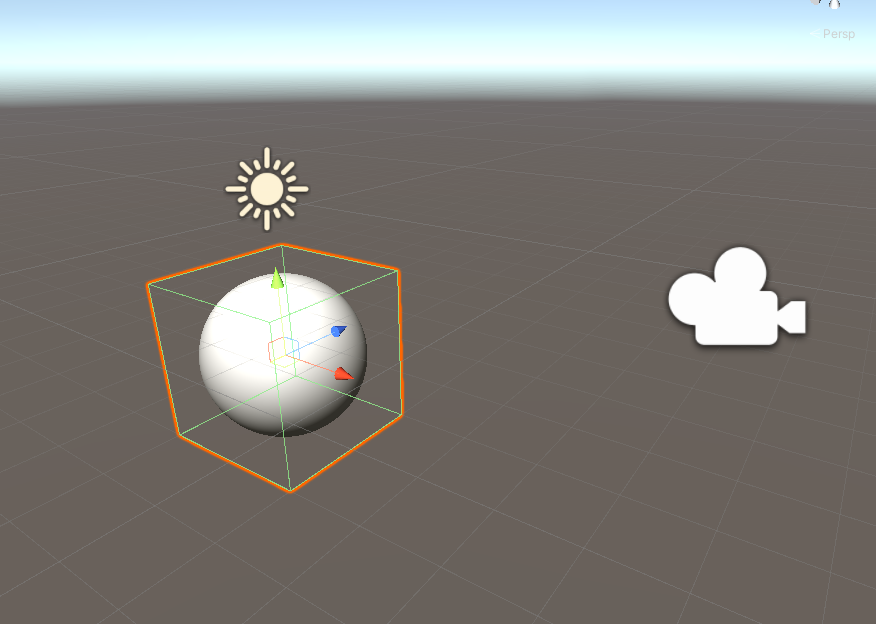
\includegraphics[width=\linewidth]{unity captures/sphere tracing shaded}
            \captionof{figure}{A 3D cube with a volumetric shader.}
            \label{img:captures:spheretracing}
        \end{minipage}
    \hfill
        \begin{minipage}{0.47\linewidth}
            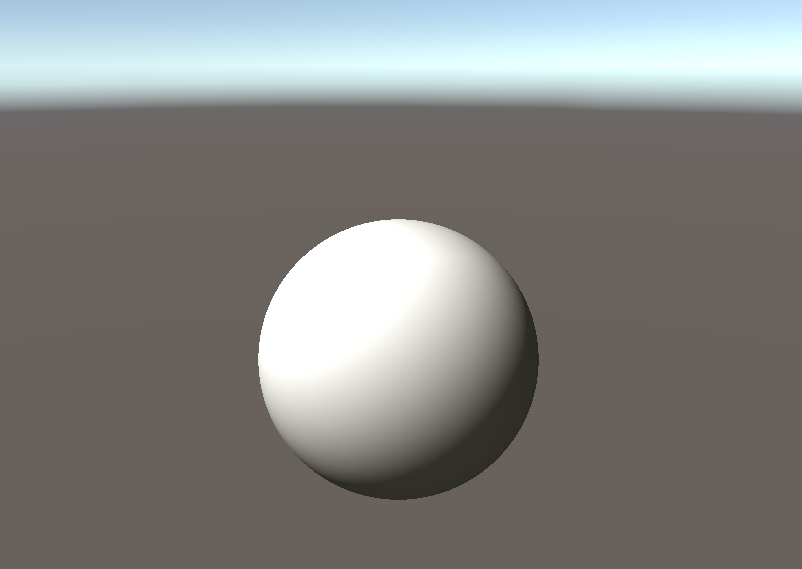
\includegraphics[width=\linewidth]{unity captures/sphere tracing shaded result}
            \captionof{figure}{The shaded sphere rendered volumetrically.}
            \label{img:captures:spheretracing_rendered}
        \end{minipage}
\end{figure}

\clearpage
\subsection{Shadow Casting}
In \gls{raymarching}, rendering cast shadows  proves to be rather easy. Naturally, the light ray comes from the sun, bounces off in the world and may eventually hit the eye of the observer.
Since only a minute fraction of those rays actually reach the observer (the camera), a huge amount of rays would be calculated for nothing.
Consequently, the rays are not traced from the light source to the camera but the other way around instead.
\\
As defined in \autoref{lst:shader:raymarch:spheretracing}, the \lstinline[language=HLSL]{raymarch()} function moves along the given ray and returns the distance to the nearest intersection of ray and volume.
Therefore, when a surface point has been determined, a second ray march can be started from the newly found point in the opposite direction the primary light source is facing. If anything is hit on the way, the surface point lies in the shadow of the second hit object and should be darkened.

\begin{figure}[H]
    \centering
    \begin{tikzpicture}[scale=1.2]
        \tikzset{edge/.style = {-{Latex[length=3mm]},shorten >= -4pt}}
        \tikzset{shadowedge/.style = {-{Latex[length=3mm]},shorten <=-4pt,shorten >= -4pt}}
        \tikzset{topshadowedge/.style = {-{Latex[length=3mm]},shorten <=-4pt}}
        \tikzset{icon/.style = {font=\Large}}

        % surf dist
        \draw[red] (5,2.5) circle (1);
        \draw[red] (-2,0) -- (7,0) -- (8,0.5);

        \node (rOrigin) at (0.2,2) {};
        \node[cyan] (r1hit) at (4.05,2.8) {\textbullet};
        \node[cyan] (r2hit) at (5.5,0) {\textbullet};
        \node[cyan] (r2light) at (5.35,1.55) {\textbullet};

        % icons
        \node (cam) at (0,2) {\faVideoCamera};
        \node[icon] (light) at (1,5) {\faLightbulbO};
        \node at (1,5.5) {light direction};
        \draw[edge] (light) -- ($ (light) - (-0.11,1) $);
        \draw[edge] ($ (light) + (0.5,0) $) -- ($ (light) + (0.61,-1) $);
        \draw[edge] ($ (light) - (0.5,0) $) -- ($ (light) + (-0.41,-1) $);

        % rays
        \draw[edge] (rOrigin) -- (r1hit) node[midway,above,sloped]{$r1$};
        \draw[topshadowedge, cyan] (r1hit) -- ($ (r1hit) + (-0.16,1.5) $) node[midway,above,sloped]{$s1$};
        
        \draw[edge] (rOrigin) -- (r2hit) node[midway,above,sloped]{$r2$};
        \draw[shadowedge, cyan] (r2hit) -- (r2light) node[midway,above,sloped]{$s2$};
        \draw[loosely dashed, cyan] (r2light) -- ($ (r2light) + (-0.16,1.5) $);

        \end{tikzpicture}
    \captionof{figure}{Shadow casting in ray marching.}
    \label{img:tikz:rendering:shadowcasting}
\end{figure}

\noindent
As seen in the figure above, the ray $r1$ hits the volumetric sphere, then checks if anything is between the ray intersection and the negative light source direction.
In this case, $s1$ does not collide with anything and the surface is shaded normally. 
For the other ray $r2$ however, the shadow ray march returns a distance $s2 > 0$ and $s2 < $\lstinline[language=HLSL]{ MAX_DISTANCE}, meaning some object is inbetween the hit point and the light source, casting a shadow.
\\
\begin{lstlisting}[language=HLSL, caption=Implementation of hard shadow casting., label=lst:shader:shadowcasting:hard]
float hardshadow(float3 position, float3 direction, float dMin, float dMax)
{
    float dOrigin = dMin;
    for (int i = 0; i < MAX_STEPS; i++) {
        float dScene = sceneSDF(position + direction * dOrigin);
        if (dScene < SURFACE_DISTANCE)
            return 0.0;
        if (dScene > dMax)
            return 1.0;
        
        dOrigin += dScene;
    }
    return 1.0;
}
\end{lstlisting}

\noindent
It is very clearly similar to SDF-based sphere tracing, except that only 0 or 1 is returned instead of the distance.
The final color is then multiplied by this output. For 0, this results in a total black, hence the name \textit{hard} shadows.

\subsubsection{Soft Shadows}
The method described in \autoref{img:tikz:rendering:shadowcasting} evaluates only if any given point is directly covered by any other object. 
It does not account for diffuse shadows with soft edges, called \textit{\gls{penumbra}} or simply \textit{soft} shadows. But there is an easy and also cost-effective solution to that problem.
Instead of strictly returning 0 when an object is covered by another, the shortest distance to scene (qualified by some factor $k$) is returned.

\begin{lstlisting}[language=HLSL, caption=Implementation of hard shadow casting., label=lst:shader:shadowcasting:soft]
float softshadow(float3 position, float3 direction, float dMin, float dMax, float k)
{
    float result = 1.0;
    float dOrigin = dMin;
    for (int i = 0; i < MAX_STEPS; i++) {
        float dScene = sceneSDF(position + direction * dOrigin);
        if (dScene < SURFACE_DISTANCE)
            return 0;
        if (dOrigin > dMax)
            return result;
        
        result = min(result, k * dScene / dOrigin);
        dOrigin += dScene;
    }
    return result;
}
\end{lstlisting}

\noindent
Those are the resulting renders with a sphere and a flat box as the volumetric scene.
\begin{figure}[H]
    \centering
        \begin{minipage}{0.3\linewidth}
            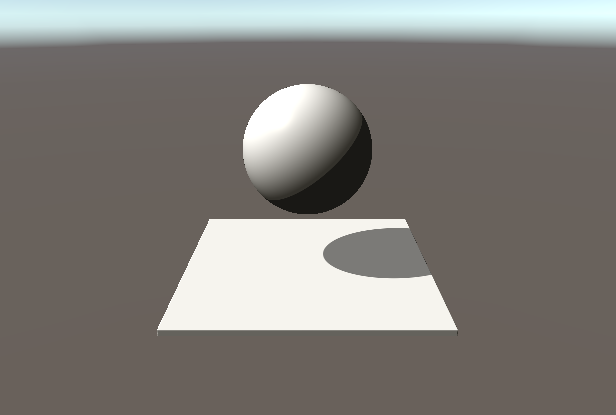
\includegraphics[width=\linewidth]{unity captures/shadow casting hard}
            \captionof{figure}{Hard shadows only.}
            \label{img:captures:shadows:hard}
        \end{minipage}
        \hfill
        \begin{minipage}{0.3\linewidth}
            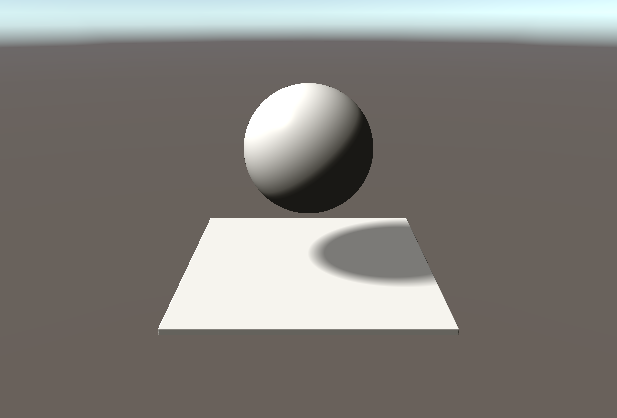
\includegraphics[width=\linewidth]{unity captures/shadow casting soft 7}
            \captionof{figure}{Soft shadows with $k=7.0$.}
            \label{img:captures:shadows:soft2}
        \end{minipage}
        \hfill
        \begin{minipage}{0.3\linewidth}
            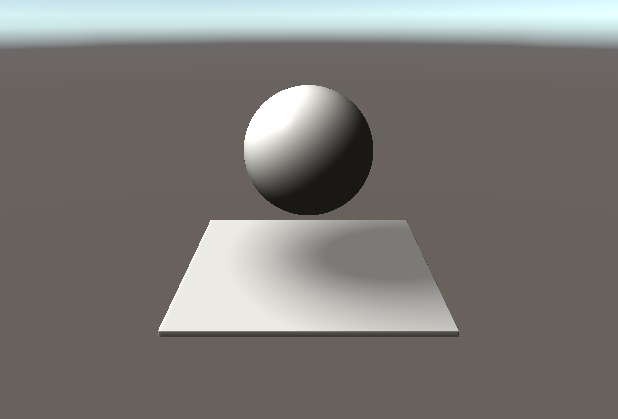
\includegraphics[width=\linewidth]{unity captures/shadow casting soft 1.2}
            \captionof{figure}{Soft shadows with $k=1.2$.}
            \label{img:captures:shadows:soft1}
        \end{minipage}
\end{figure}

\clearpage
\subsection{Shape Blending}
Another thing that comes free with ray marching is \textit{\gls{shapeblending}}. It describes the concept of blending the \gls{sdf}s of mulitple shapes together with this simple method:
\begin{lstlisting}[language=HLSL]
float blend(float d1, float3 d2, float k)
{
    return k * d1 + (1 - k) * d2;
}
\end{lstlisting}

\noindent
Now two shapes can simply be blended like that:
\begin{lstlisting}[language=HLSL]
float sceneSDF(float3 position)
{
    return blend(sphereSDF(position), boxSDF(position), 0.5);
}
\end{lstlisting}

\noindent
The following image displays the two blended shapes. Due to the fact that the shadow is calculated live, no additional changes have to be made in this regard.
\begin{figure}[H]
    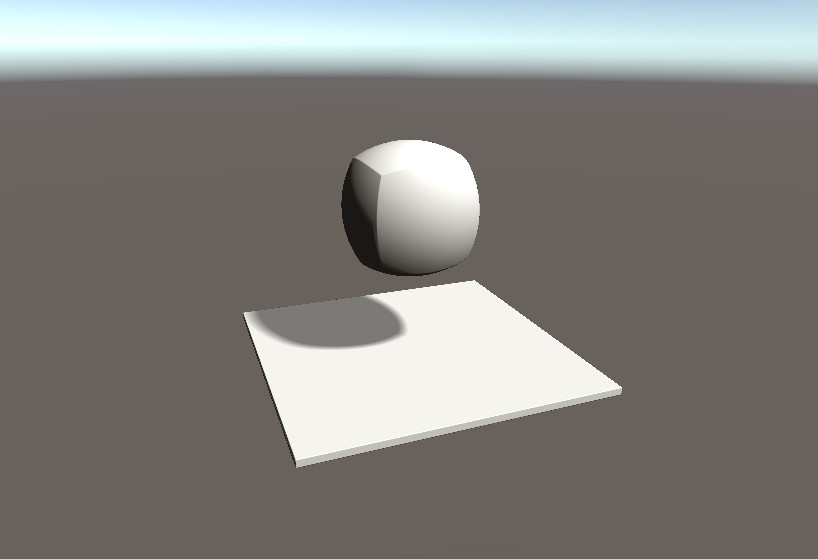
\includegraphics[width=\linewidth]{unity captures/shape blending 1}
    \captionof{figure}{A blended sphere and box SDF with $k = 0.5$.}
    \label{img:captures:shapeblending1}
\end{figure}

\clearpage
\subsubsection{Solid Primitive Operators}
To create more interesting figures than a rounded box, solid primitive operators can be used. As seen in \autoref{img:captures:shapeblending2}, "holes" are cut into the geometry. This is done by taking the difference (or intersection) of the box and a cylinder that goes through the box.
Like the \lstinline[language=HLSL]{blend()} function takes in two \gls{sdf} results, the following methods also compare the distances.

\begin{lstlisting}[language=HLSL, caption=Implementation of solid primitive operations., label=lst:shader:shapeblending:primitiveoperations]
float intersection(float d1, float d2)
{
    return max(d1, d2);
}

float union(float d1, float d2)
{
    return min(d1, d2);
}

float difference(float d1, float d2)
{
    return max(d1, -d2);
}
\end{lstlisting}

\noindent
In this example, the intersection was done three times, for each axis once.

\begin{figure}[H]
    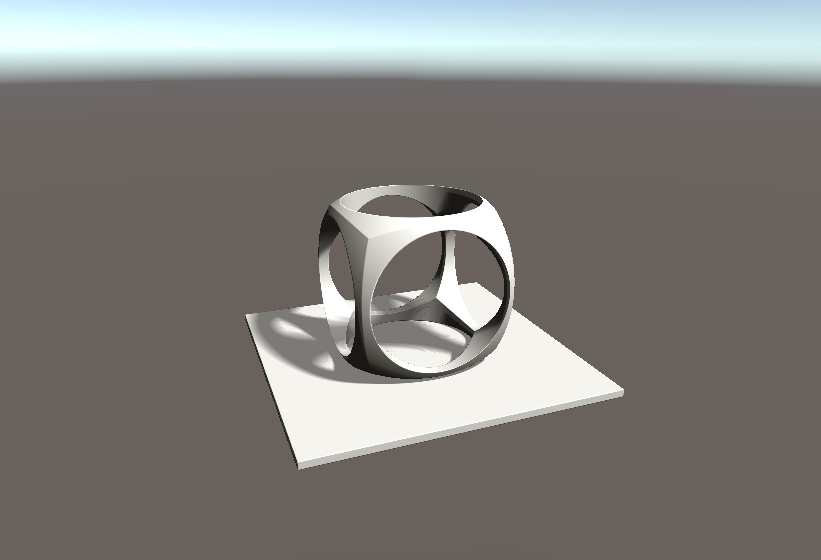
\includegraphics[width=\linewidth]{unity captures/shape blending 2}
    \captionof{figure}{A blended sphere and box with holes along each axis.}
    \label{img:captures:shapeblending2}
\end{figure}

\clearpage
\subsection{Ambient Occlusion}
Shadow casting already looks quite realistic, but there is an important detail missing, called \textit{\gls{ambientocclusion}}. This method darkens areas around edges and crevices in the scene, making them look less exposed to the light and its environment.
The algorithm for that is fairly uncomplicated and straightforward, given all the previously defined methods like \lstinline[language=HLSL]{sceneSDF()} and \lstinline[language=HLSL]{raymarch()} already exist.
\\
When the \lstinline[language=HLSL]{raymarch()} function returns a valid distance, a surface is hit. On that hit point $p_1$, the normal vector $\overrightarrow{n}$ is estimated. Now the distance to the nearest surface in the direction of $\overrightarrow{n}$ is evaluated.
If on that ray a hit point $p_2$ is close, the color for the original hit point $p_1$ is darkened by some amount, depending on how far apart those points are.

\begin{lstlisting}[language=HLSL, caption=Implementation of ambient occlusion., label=lst:shader:ambientocclusion]
float ambientOcclusion(float3 p, float3 direction) {
    float ao = 0;
    float dOrigin = 0;

    for (int i = 1; i <= AO_ITERATIONS; i++) {
        dOrigin = AO_STEP_SIZE * i;
        ao += max(0, dOrigin - sceneSDF(p + direction * dOrigin)) / dOrigin;
    }
    return 1 - ao * AO_INTENSITY;
}
\end{lstlisting}

\noindent
This comes close to the constant step ray marching algorithm, since it is marched along the ray in a predefined step size.
On line 7, the scene SDF is substracted from the total distance and then devided by it. This just puts the scene distance in relation to the total distance.
Also, \lstinline[language=HLSL]{max()} is used because the SDF can return a negative number for points inside the surface, so in order to not brighten the scene at point \lstinline[language=HLSL]{p} when this is the case, 0 is added instead.
\\
With \lstinline[language=HLSL]{AO_STEP_SIZE = 0.1}, \lstinline[language=HLSL]{AO_ITERATIONS = 3} and \lstinline[language=HLSL]{AO_INTENSITY = 0.2}, the following output is produced.

\begin{figure}[H]
    \centering
        \begin{minipage}{0.47\linewidth}
            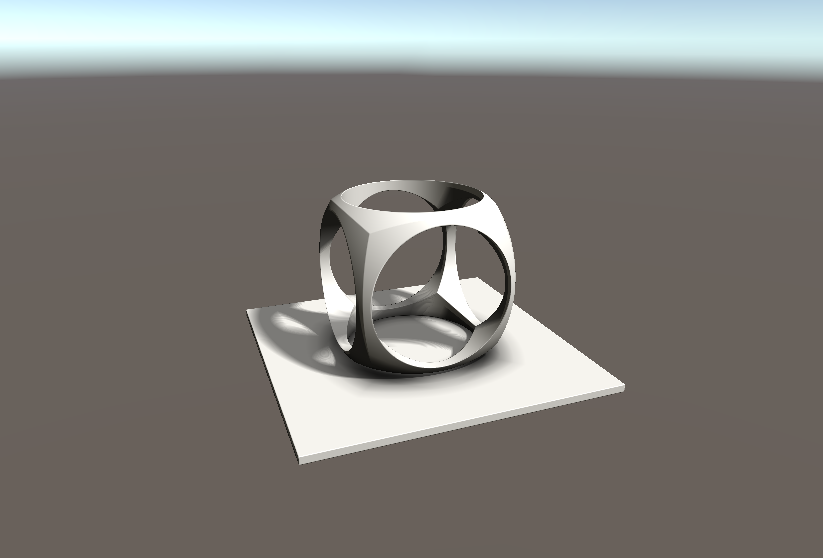
\includegraphics[width=\linewidth]{unity captures/ambient occlusion ON}
            \captionof{figure}{Ambient occlusion applied to the scene.}
            \label{img:captures:ambientocclusion:on}
        \end{minipage}
    \hfill
        \begin{minipage}{0.47\linewidth}
            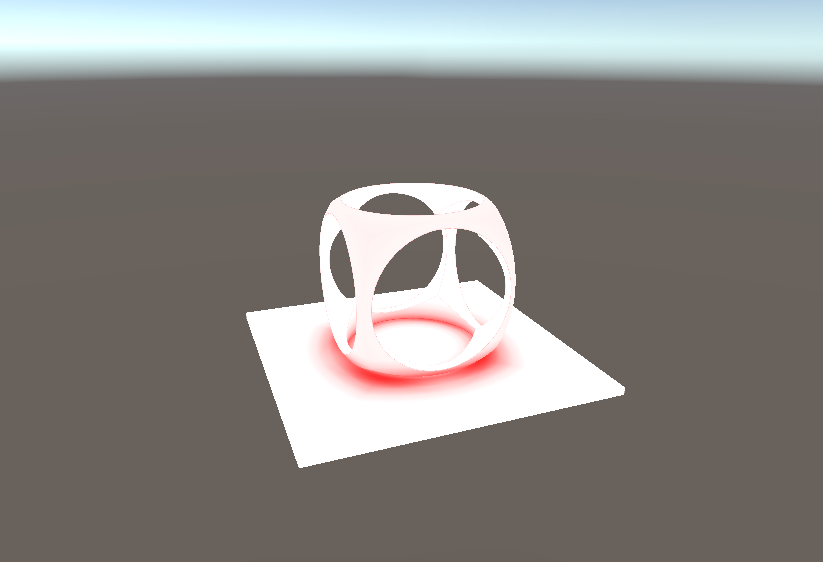
\includegraphics[width=\linewidth]{unity captures/ambient occlusion only}
            \captionof{figure}{Only the ambient occlusion part drawn in red.}
            \label{img:captures:ambientocclusion:only}
        \end{minipage}
\end{figure}

\noindent
When comparing the previous \autoref{img:captures:shapeblending2} with \autoref{img:captures:ambientocclusion:on}, the darker ground around the object clearly improves the scene.